\subsubsection{$t+\met$ final state}
\label{sec:monotop}
 
The search performed during the LHC Run 1 with the ATLAS experiment for the production of 
single-top quarks in association with missing energy denoted as monotop is briefly described in this section,
for more information see Ref.~\cite{ATLASmonotop}. 
The search is based on the lepton+jets channel where the $W$ boson coming from the top quark decays leptonically 
into an electron or a muon in association with a neutrino.
The experimental signature of monotop events is given by one isolated charged lepton (electron or muon),
large missing transverse energy, and one $b$-tagged jet as shown in Fig.~\ref{fig:feyn_prod_lepdecay}.

\begin{figure}[!h!tpd]
\centering
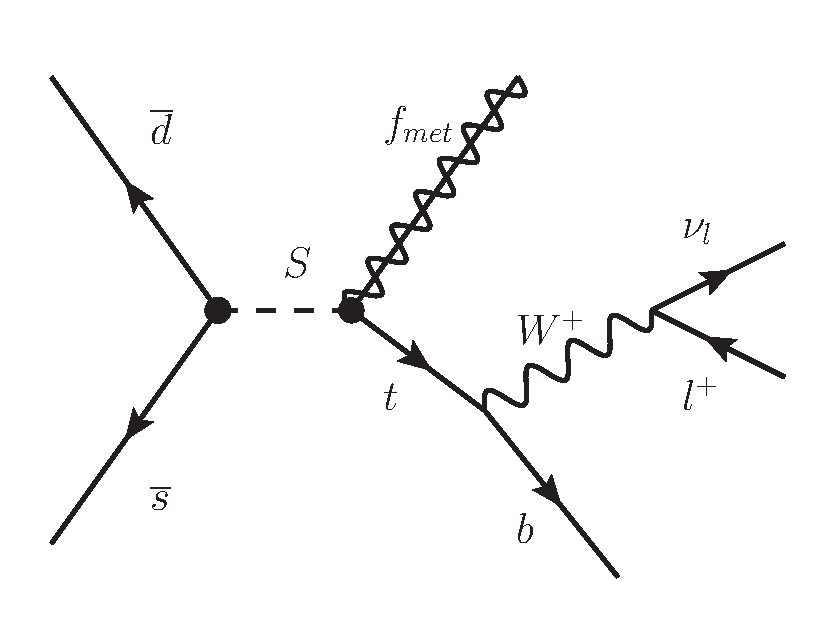
\includegraphics[width=0.31\textwidth]{feyn_diags/S1_leptopdecay}
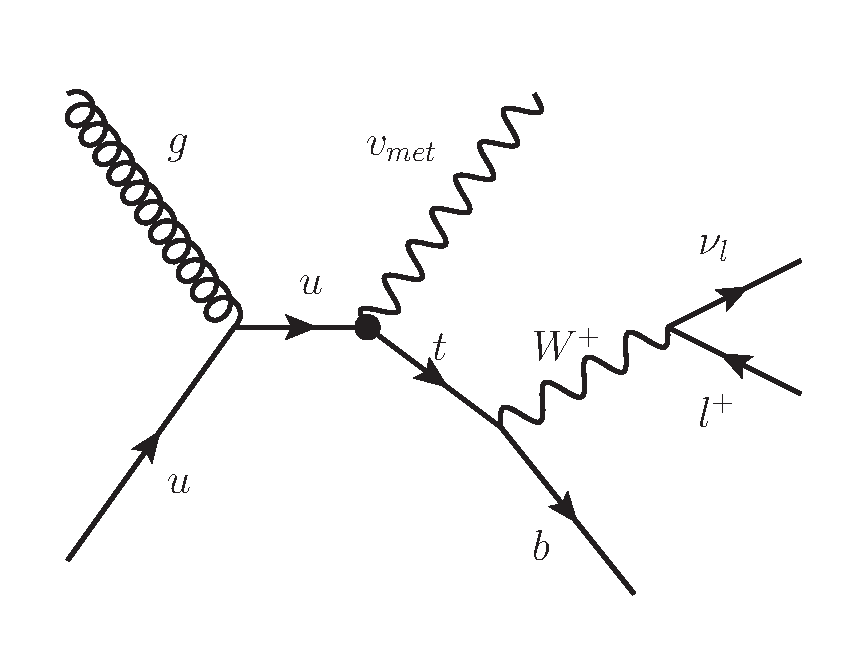
\includegraphics[width=0.31\textwidth]{feyn_diags/S4_s_leptopdecay}
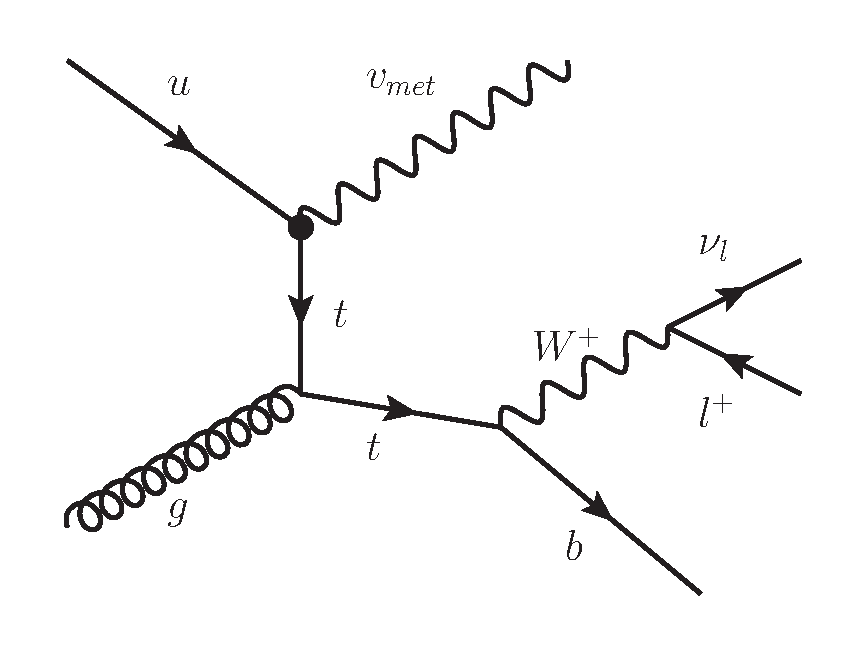
\includegraphics[width=0.31\textwidth]{feyn_diags/S4_t_leptopdecay}
%\subfigure[\label{subfig:S1_leptopdecay}]{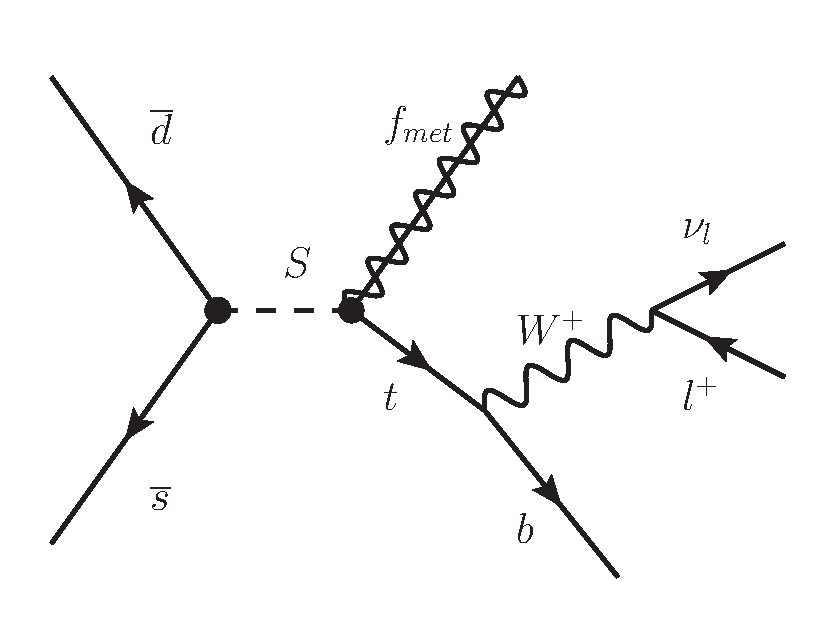
\includegraphics[width=0.46\textwidth]{feyn_diags/S1_leptopdecay}}\\
%\subfigure[\label{subfig:S4_s_leptopdecay}]{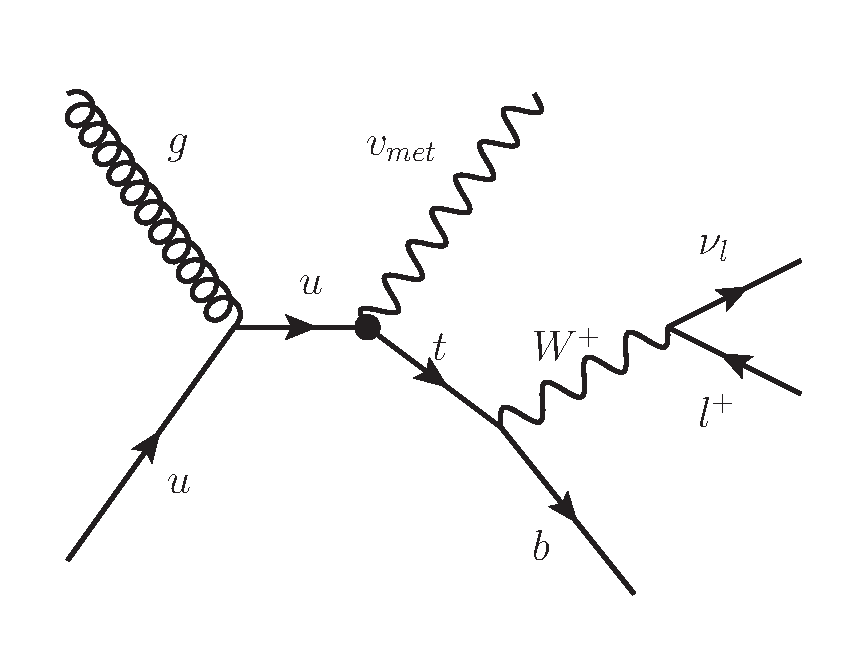
\includegraphics[width=0.46\textwidth]{feyn_diags/S4_s_leptopdecay}}
%\subfigure[\label{subfig:S4_t_leptopdecay}]{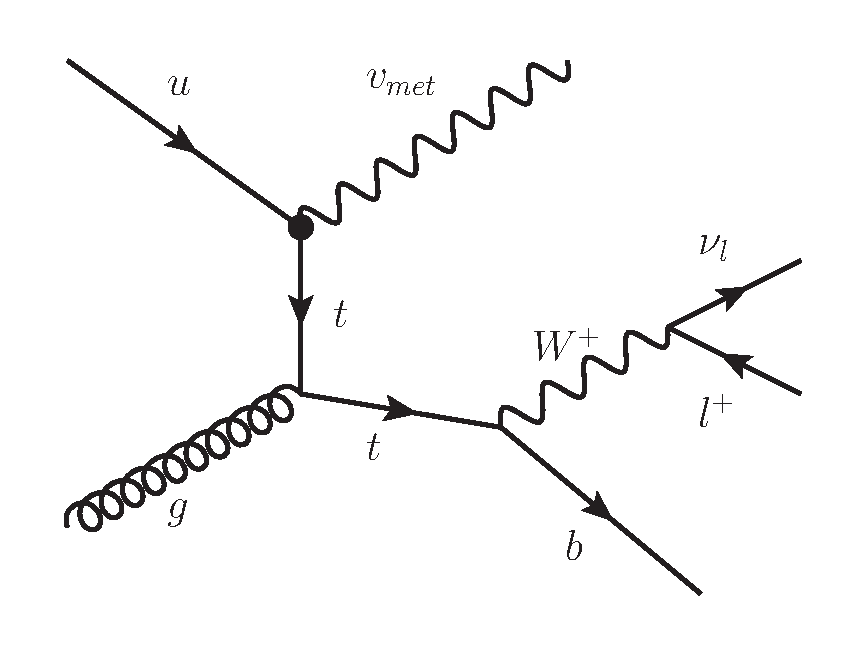
\includegraphics[width=0.46\textwidth]{feyn_diags/S4_t_leptopdecay}}
\caption
{
Feynman diagram of leading order processes leading to monotop events with a semi-leptonic topology: production of
a coloured scalar resonance $S$ decaying into a top quark and a spin-$1/2$ fermion $f_{met}$
in the resonance model, and $s$- and $t$-channel non resonant production of a top quark in association with
a spin-1 boson $v_{met}$ in the non-resonance model.
%Feynman diagram of leading order processes leading to monotop events with a semi-leptonic topology: production of
%a coloured scalar resonance $S$ decaying into a top quark and a spin-$1/2$ fermion $f_{met}$
%in the $\mathrm{S1_R}$ model~\subref{subfig:S1}, and $s$-\subref{subfig:S4_s}
%and $t$-\subref{subfig:S4_t} channel non resonant production of a top quark in association with
%a spin-1 boson $v_{met}$ in the $\mathrm{S4_R}$ model.
}
\label{fig:feyn_prod_lepdecay}
\end{figure}

The analysis strategy used in this search is based on a cut-and-count approach which is used to extract the 
monotop signal. The azimuthal angle difference between the charged lepton and the $b$-jet ($|\Delta \phi(l,b)|$) 
and low transverse W mass ($m_\mathrm{T}(W)$) are used to define the final signal regions: 
\begin{itemize}
  \item For the resonant case, the optimized signal region is $m_\mathrm{T}(W)>210\mathrm{~GeV}$ and $|\Delta \phi(l,b)|<$~1.2 in addition to the signal region pre-selection
  
  \item For the non-resonant case, the optimized signal region is $m_\mathrm{T}(W)>250\mathrm{~GeV}$ and $|\Delta \phi(l,b)|<$~1.4 in addition to the signal region pre-selection

\end{itemize}
The main background contributions to the signal regions is the top-antitop quark pair production ($t\bar{t}$)
in particular dilepton $t\bar{t}$ events.
The main systematic uncertainties are those related to the jet energy scale, the b-tagging efficiency, the effect of the choice of PDF on signal and background 
acceptance, the effect of the choice of Monte Carlo (MC) generator and of additional radiation on $t\bar{t}$ modelling, and the effect of the limited size of the samples.

In the absence of deviation with respect to the SM predictions,
this search gives upper limits on the production cross-section at 95\% confidence level (CL)
for two signal models, producing right-handed top quarks together with exotic objects
giving rise to missing energy.
In the case of the production of a 500~GeV spin-0 resonance, the excluded effective coupling is below \ares=~0.15,
for a mass of the invisible spin-1/2 state between 0 and 100~GeV.
In the case of non-resonant production, the \anonres=~0.2 effective coupling is excluded
for a mass of the invisible spin-1 state between 0 and 650~GeV. 

The monotop search in the hadronic channel will be considered in Run 2.

 \subsubsection{$tt+X$ final state}
 
 The main feature of this final state is two particles with the same electric charge. In order to exploit this point,it is essential to consider the events where both top quarks decay into leptons. 
 The relevant final state probing this model is then $\ssll + X$, where $X$ depends on the exact process ($X=j + 2b$-jets for all diagrams of 
 Figures~\ref{fig:feyn_prod_ss_real} and~\ref{fig:feyn_prod_ss_virt} but the $t$-channel, $X=2 b$-jets for the $t$-channel of Figure~\ref{fig:feyn_prod_ss_virt}).
 The cross-sections involving valence quarks are higher than the ones involving see quarks. Thus, the positively charged top quark pairs are largely more produced.

\begin{figure}[!h!tpd]
\centering
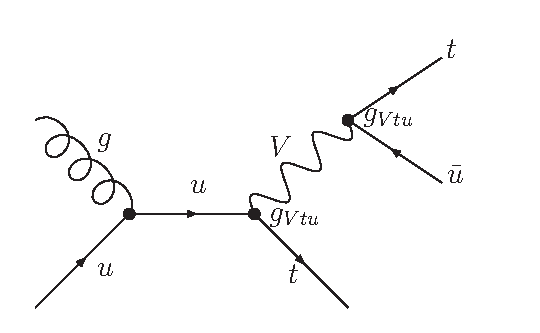
\includegraphics[width=0.35\textwidth]{feyn_diags/gu_Vt_tu}  \hspace{1.5cm}
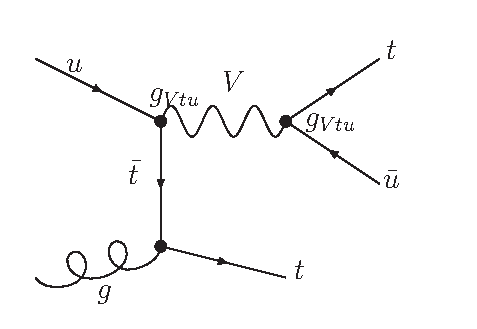
\includegraphics[width=0.32\textwidth]{feyn_diags/gu_Vt_tu_2}
\caption
{
Feynman diagram of leading order processes leading to the $tt\bar{u}$ via the $V$ production and its decay into $t\bar{u}$.
}
\label{fig:feyn_prod_ss_real}
\end{figure}

\begin{figure}[!h!tpd]
\centering
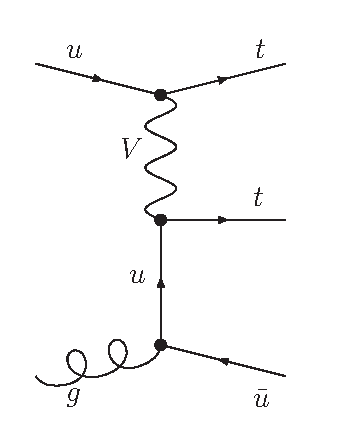
\includegraphics[width=0.21\textwidth]{feyn_diags/other_gu_ttu} \hspace{3.5cm}
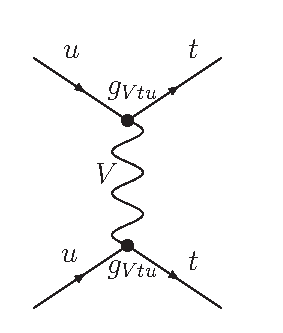
\includegraphics[width=0.21\textwidth]{feyn_diags/uu_tt}
\caption
{
Feynman diagram of leading order processes leading to the $tt\bar{u}$ (left) and to the $tt$ production (right), both via $V$ exchange in the $t$-channel.
}
\label{fig:feyn_prod_ss_virt}
\end{figure}

 The typical background for this final state is mainly instrumental via a wrong charge reconstruction but can also be physical. Indeed, the $\ttbarV$ production can yield to a same-sign 
lepton pair together with $b$-jets. On the other hand, the $\ttbar$ production is large enough to make the charge mis-reconstruction rate relevant. Finally,``trident'' electrons 
(photon radiation and conversion) can also contribute to this final state.

The Run 1 analysis exploiting the $\ssll+b-$jets signature~\cite{ATLASsamesigntop} is able to exclude a 
typical cross-section of $10$~fb for a FCNC Higgs signal (similar to the $tt$ production of Figure~\ref{fig:feyn_prod_ss_virt}). 
Given the cross-sections of the described model, this final state is quite sensitive
to a wide range of parameters.% \com{reference to the appendix of $\sigma(tt\bar{u}+tt)$ cross-sections, in appendix}.

There is one particular feature, not yet exploited, that can be used to extract the $tV(\to t\bar{u})$ production: the transverse momentum of the leading jet is quite high 
and will definitely help to disentangle the signal and the SM backgrounds, further increasing the sensitivity of this channel. As a consequence, the results shown
in section~\ref{sec:comb} are quite conservative.
%\com{Add $p_T$ leading jet distribution for 2 signals and SM backgrounds}. 

 
 \subsubsection{Combination of $tt+X$ and $t+\met$ analysis for the non-resonant production}
 \label{sec:comb}
 
 The interesting point in combining the $tt$ and $t+\met$ analysis is to cover invisible and the visible $V$ decay simultaneously. The visible decay must 
 be taken into account simply because $V$ is produced from visible particles. More the production is large, more the visible decay should be relevant. 
 In order to see the interplay, it is necessary to express the two constraints in the same parameter space.

 Assuming that the phenomenology is fully described by $\sigma_{tV}$, $\sigma_{tt}$, $\sigma^{\rm{virt}}_{tt\bar{u}}$ and $\BR{V}{\chi\chi}$, 
 the experimental cross-sections for each final state can be predicted:
 \begin{eqnarray}
   \sigma_{t+\met} &=& \sigma_{tV} \times \BR{V}{\chi\chi} \label{eq:ExpCrossSectiont} \\
   \sigma_{tt+X}   &=& \sigma_{tV} \times \frac{1-\BR{V}{\chi\chi}}{2} \; + \; \sigma^{\rm{virt}}_{tt\bar{u}} \;+\; \sigma_{tt}    \label{eq:ExpCrossSectiontt}
 \end{eqnarray}
 where $\sigma_{tV}$ correspond to the $2$ diagrams of Figure~\ref{fig:feyn_prod_ss_real}, $\sigma^{\rm{virt}}_{tt\bar{u}}$ ($\sigma_{tt}$) 
 corresponds to the left (right) diagram of Figure~\ref{fig:feyn_prod_ss_virt}.\com{IMPORTANT COMMENT: this split is in principle not correct, but needed. Not
 correct because all $gu \to tt\bar{u}$ amplitudes must interfere. Needed because only the real production is scaled by $\BR{V}{\chi\chi}$, in which we are precisely interested.
 This needs to be further discussed with theorists.} The factor $2$ comes from the fact that $\BR{V}{t\bar{u}} = \BR{V}{\bar{t}u}$. 
 In practice, the selection efficiency will be different for each process, since they have quite different topology. We neglect this aspect in this simplified discussion.

 If we neglect the term $\sigma^{\rm{virt}}_{tt\bar{u}} \:+\: \sigma_{tt}$ in equation~\eqref{eq:ExpCrossSectiontt}, it becomes easy to compute the excluded area in
 the plane $(\sigma_{tV}, \BR{V}{\chi\chi})$ by each of the channel. Considering the excluded cross-section in the monotop analysis ($\sigma^{\rm{excl}}_{t+\met}$) 
 and in the same-sign top analysis ($\sigma^{\rm{excl}}_{tt+X}$), it comes:
 \begin{eqnarray}
  \label{eq:ExclusionArea}
  \left( \sigma^{\rm{excl}}_{tV} \right)_{\rm{monotop}} &>& \frac{\sigma^{\rm{excl}}_{t+\met}}{\BR{V}{\chi\chi}} \label{eq:ExclusionArea1} \\
  \left( \sigma^{\rm{excl}}_{tV} \right)_{\rm{sstop}}   &>& \frac{2\times\sigma^{\rm{excl}}_{tt+X}}{1-\BR{V}{\chi\chi}} \label{eq:ExclusionArea2}
 \end{eqnarray}

 According to the monotop and same-sign top analysis performed during the Run 1, the cross-sections limits for $m_V \sim 500$~\GeV{} are:
 \begin{eqnarray}
  \sigma^{\rm{excl}}_{t+\met} \times \BR{W}{\ell\nu_{\ell}} &\sim& 250~\rm{fb}\\
  \sigma^{\rm{excl}}_{tt+X}   &\sim&  10~\rm{fb}
 \end{eqnarray}

 By putting these numbers into equations~\eqref{eq:ExclusionArea1} and~\eqref{eq:ExclusionArea2} ($\BR{W}{\ell\nu_{\ell}}$ include electrons and muons only and is taken at $21.3\%$), 
 we obtain the excluded areas in the $(\sigma_{tV},\BR{V}{\chi\chi})$ plane for each analysis as shown in figure~\ref{fig:Limit}.
 The power of the same-sign signature offers a nice way to complete the monotop analysis for $\BR{V}{\chi\chi} \lesssim 0.98$ and to exclude a much larger part of the parameter space.

 \begin{figure}[htbp]
  \centering
  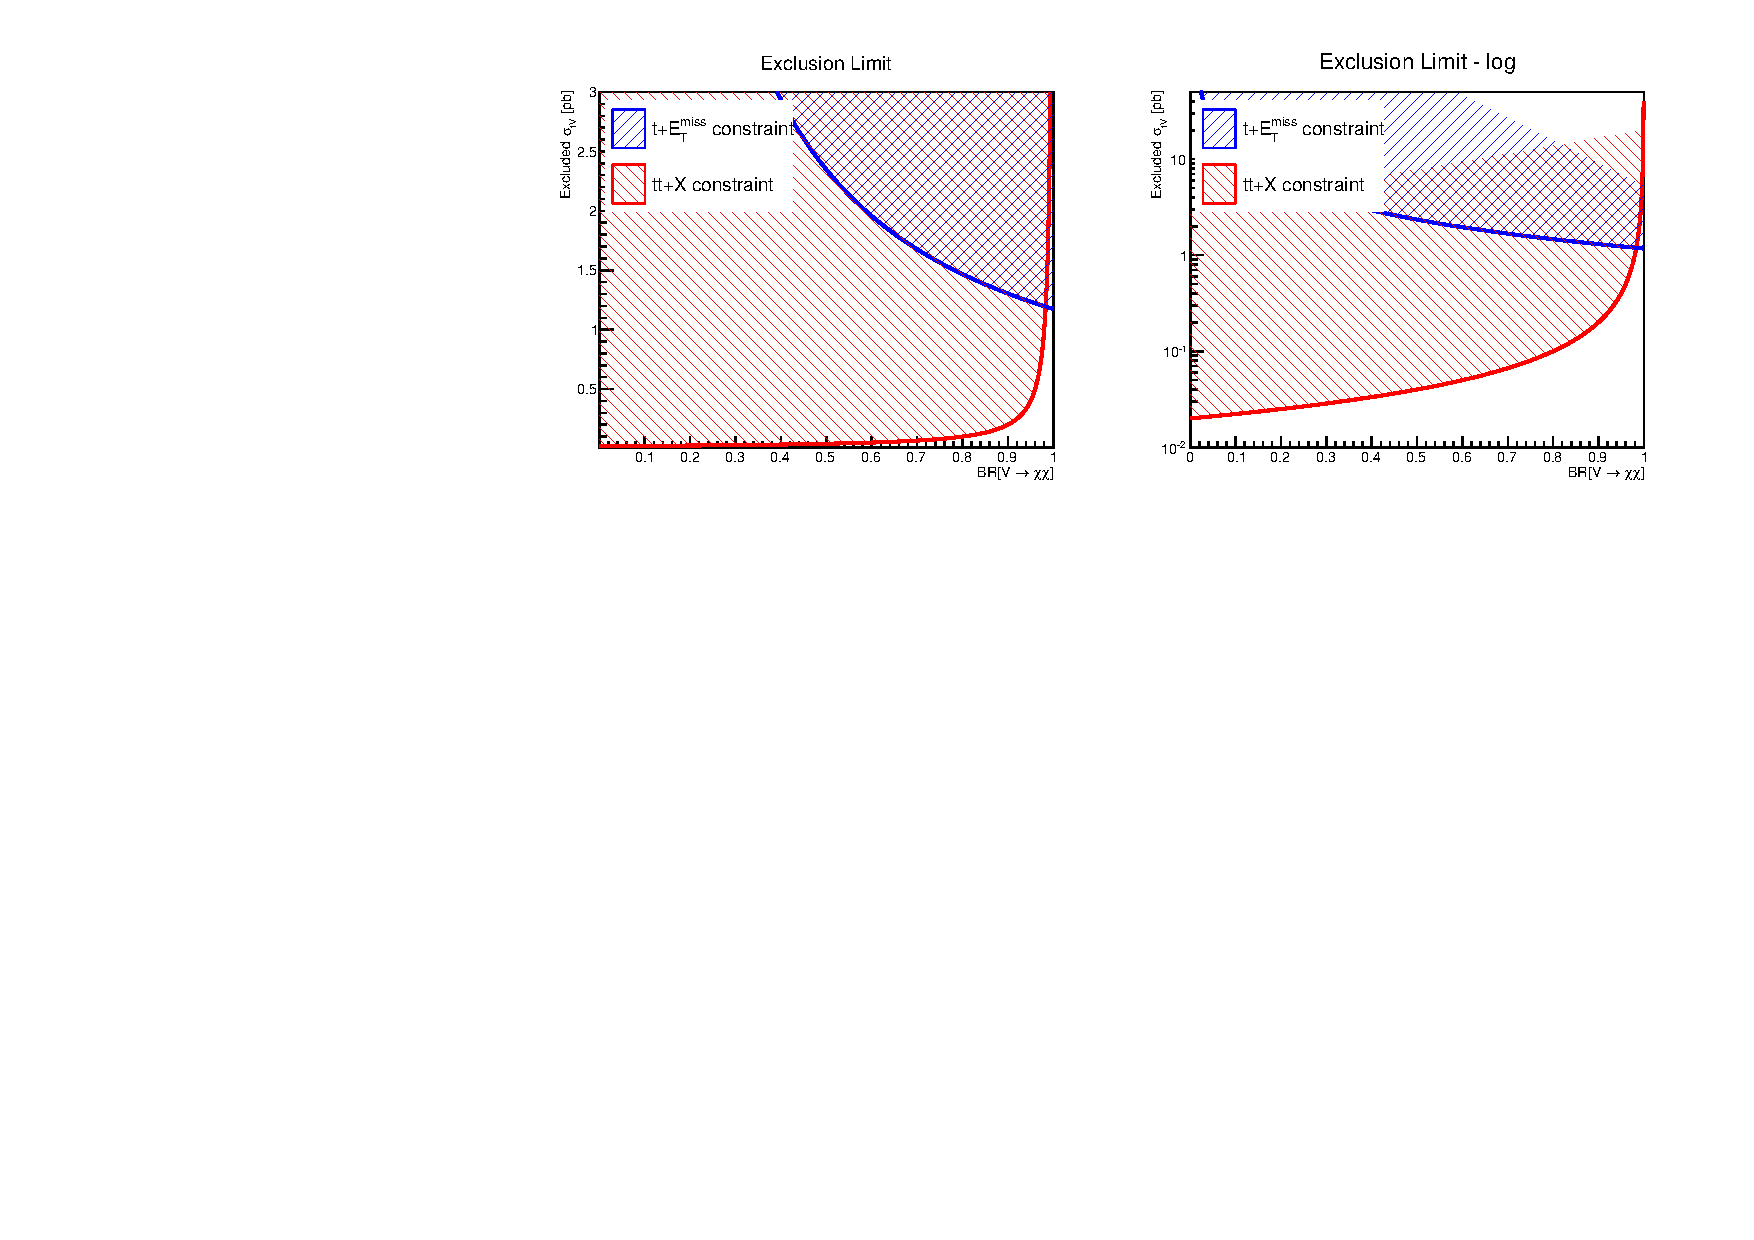
\includegraphics[width=1.0\columnwidth]{Limit}
  \caption{All cross-sections above the curves are excluded cross-section by the monotop analysis (blue) and the $\ssll$ (red) as a function of $\BR{V}{\chi\chi}$. For $\BR{V}{\chi\chi}\lesssim 0.98$, 
  the monotop only excludes large cross-sections while the $\ssll$ takes over in order to recover some sensitivity.}
  \label{fig:Limit}
\end{figure}

In practice, equations~\eqref{eq:ExpCrossSectiont} and~\eqref{eq:ExpCrossSectiontt} show that figure~\ref{fig:Limit} underestimate the sensibility of the $tt+X$ analysis since the terms 
$\sigma^{\rm{virt}}_{tt\bar{u}}$ and $\sigma_{tt}$ were neglected. The additional sensitivity brought by these terms might depend on the event selection, due
to the different event topology (for instance, leading jet softer). Also, the way to interpret the two analysis in the same parameter plane becomes less obvious
when $\sigma^{\rm{virt}}_{tt\bar{u}}$ and $\sigma_{tt}$ are involved. In this case, the couplings $g^{R}_{Vtu}$ and $m_V$ might be a good option but this has to
be properly defined \com{Need discussion with theorists}.
